\documentclass[12pt]{article}

% Packages
\usepackage{graphicx}
\usepackage{subcaption}
\usepackage{hyperref}

\usepackage[margin=1in]{geometry}

% Translations

\ifdefined\swedish
    \newcommand{\text}[2]{#2}
\else
    \newcommand{\text}[2]{#1}
\fi

\graphicspath{{./graphics/}}

\pagenumbering{gobble}
\usepackage[utf8]{inputenc}

\begin{document}

\begin{figure*}
    \begin{subfigure}[]{0.4\textwidth}
        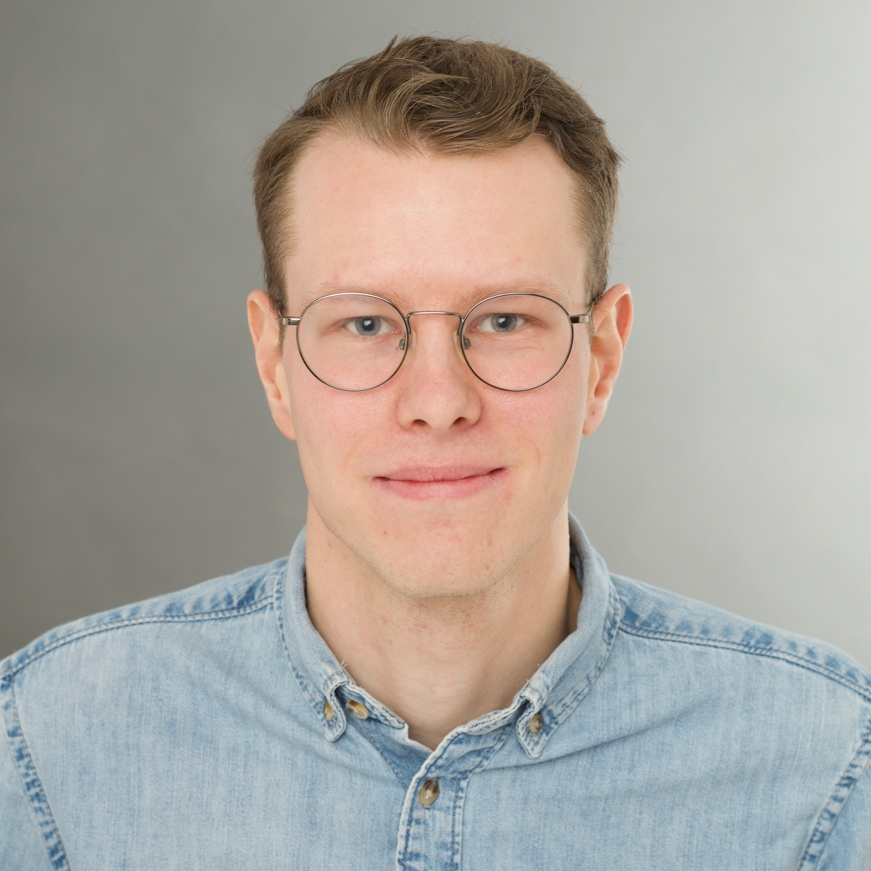
\includegraphics[height=6cm]{photo}
    \end{subfigure}%
    ~
    \begin{subfigure}[]{0.5\textwidth}
        \part*{Joel Oskarsson}

        \begin{tabular}{l l}
            \href{mailto:\email}{\email} & \text{+46706724739}{0706724739}\\
            \href{http://joeloskarsson.github.io}{joeloskarsson.github.io} & \href{http://linkedin.com/in/joel-oskarsson}{linkedin.com/in/joel-oskarsson}\\
        \end{tabular}
        \\
        \\

        \begin{tabular}{l l}
            Dept. of Computer and Information Science & \\
            Linköpings universitet & \\
            SE-581 83 Linköping, Sweden & \\
        \end{tabular}

     \end{subfigure}%
\end{figure*}

\section*{\text{Education}{Utbildning}}
\begin{itemize}
    \item \text{
            In progress: \textbf{Doctoral Studies in Computer Science, Linköping University}, Linköping, 240 ECTS\\
        Aug 2020 --
            %In the general area of statistical machine learning. Research focused on machine learning for spatio-temporal problems.
            \begin{itemize}
                \item Part of the Division of Statistics and Machine Learning, Department of Computer and Information Science. I am supervised by \href{https://lindsten.netlify.app/}{Fredrik Lindsten} (main), \href{https://liu.se/en/employee/persi28}{Per Sidén} and \href{https://www.ida.liu.se/~jospe50/}{Jose M. Peña}
                   \item In my research I develop machine learning methods for data with spatial-, temporal- and graph-structure, including combinations of these. I am interested in how more traditional probabilistic methods in these domains can be combined with deep learning in order to derive new methods with useful properties.
                   \item I am an affiliated PhD Student in the \href{https://wasp-sweden.org/}{Wallenberg AI, Autonomous Systems and Software Program}
            \end{itemize}
        }{
            Pågående: \textbf{Doktorandstudier i Datalogi}, Linköping, 240 HP\\
            aug 2020 -- \\
            Inom området statistisk maskininlärning. Forskning fokuserad på maskininlärning för spatio-temporala problem.
        }
    \item \text{
            \textbf{Master programme in Computer Science and Engineering (Swedish Civilingenjörsprogram), Linköping University}, Linköping, 300 ECTS\\
        Aug 2015 -- June 2020\\
        }{
            \textbf{Civilingenjörsprogram i Datateknik, Linköpings Universitet}, \\ Linköping, 300 HP\\
        aug 2015 -- juni 2020\\
        }
        \text{
            Bachelor courses in mathematics, programming and electrical engineering. Master focused on machine learning, statistics and AI.
        }{
            Kurser på kandidatnivå inom matematik, programmering och hårdvara. Masterprofil inom artificiell intelligens och maskininlärning.
        }
        \begin{itemize}
            \item \text{
                    Master thesis: \href{http://urn.kb.se/resolve?urn=urn:nbn:se:liu:diva-166637}{Probabilistic Regression using Conditional Generative Adversarial Networks}
                }{
                    Master-uppsats: \href{http://urn.kb.se/resolve?urn=urn:nbn:se:liu:diva-166637}{Probabilistic Regression using Conditional Generative Adversarial Networks}
                }
        \end{itemize}

    \item \text{
            \textbf{Exchange Year, ETH Zürich}, Zürich, Switzerland\\
        Sep 2018 -- Aug 2019\\
        }{
            \textbf{Utbytesår, ETH Zürich}, Zürich, Schweiz\\
        sep 2018 -- aug 2019\\
        }
        \text{
            First year of my master as an exchange student at ETH. Courses mainly in machine learning and AI.
        }{
            Första året av masterstudier vid ETH. Kurser främst inom AI och maskininlärning.
        }

\end{itemize}

\section*{\text{Employment}{Anställningar}}
\begin{itemize}
    \item \textbf{\text{PhD Student, Linköping University}{Doktorand, Linköpings Universitet}}, Linköping\\
    Aug 2020 --\\
    At the Division of Statistics and Machine Learning, Department of Computer and Information Science.

    \item \textbf{\text{Teaching Assistant, Linköping University}{Kursassistent, Linköpings Universitet}}, Linköping\\
        \text{Multiple periods}{Flera perioder} 2016--2019\\
        \text{
            Held lessons, seminars and lab-sessions for courses in mathematics, computer science and machine learning. Developed my teaching skills and my ability to communicate scientific concepts.
        }{
            Hållit i lektioner, seminarier och laborationer för kurser inom matematik, datavetenskap och maskininlärning. Har utvecklat mina pedagogiska egenskaper och min vana att kommunicera vetenskapliga koncept.
        }
    \item \textbf{Summer Intern, Ericsson}, Linköping\\
        Jun-Aug 2018\\
        \text{
            Summer internship at Ericsson Research. Worked with GNSS positioning.
        }{
            Sommarjobb vid Ericsson Research. Arbetade med GNSS-positionering.
        }

\end{itemize}

\section*{\text{Specific Knowledge}{Specifika Kunskaper}}
\begin{itemize}
        \item \text{
                Models and algorithms for modern \textbf{machine learning and AI} applications. Including, but not limited to:
        \begin{itemize}
            \item Deep learning models, advanced architectures and training regimes
            \item Bayesian models and inference methods
            \item Underlying statistical theory
            \item Implementations using suitable libraries
        \end{itemize}
        }{
            Konkreta kunskaper om relevanta modeller och algoritmer inom modern \textbf{maskininlärning och AI}. Inkluderar bl.a.:
        \begin{itemize}
            \item Olika modeller baserade på neurala nätverk
            \item Underliggande teori inom matematisk statistik
            \item Implementation med lämpliga mjukvaru-bibliotek
        \end{itemize}
        }

\item \text{Programming languages and frameworks}{Programmeringsspråk och ramverk}
        \begin{description}
            \item [\text{Knowledgeable in}{Goda kunskaper}] Python, PyTorch \text{and}{och} SciPy/NumPy.
            \item [\text{Experience with}{Erfarenhet av}] Tensorflow, R, scikit-learn, Java, MATLAB \text{and}{och} C++.
        \end{description}

    \item \text{
            Accustomed to working in Linux environments.
        }{
            Stor vana av att arbeta i Linux-miljöer.
        }

    \item \text{
            Speak both Swedish and English fluently and communicate well in both languages. Basic understanding of German.
        }{
            Pratar både svenska och engelska flytande och kan kommunicera väl på båda språken. Grundläggande förståelse av Tyska.
        }

\end{itemize}

\iffalse
\section*{\text{Other Experiences}{Övriga Erfarenheter}}
\begin{itemize}
    \item \text{
            Experience with \textbf{competitive programming}. Competed in the IMPA competition at Linköping University with good results. I have also taken part in the Nordic Collegiate Programming Contest. This has given me good training in algorithm construction and testing.
        }{
            Hållit på med \textbf{tävlingsprogrammering}. Deltagit i tävlingen IMPA på Linköpings Universitet med goda resultat, samt programmerings-SM. Givit bra erfarenheter av algoritmkonstruktion och testning.
        }

    \item \text{
            Developed multiple \textbf{hobby projects} such as smaller programs and video games. Some of these, as well as some university assignments, can be found on my \href{http://github.com/joeloskarsson}{GitHub}.
        }{
            Utvecklat många \textbf{hobbyprojekt}, så som mindre program och spel. Vissa av dessa, samt en del uppgifter från universitetskurser, hittas på min \href{http://github.com/joeloskarsson}{GitHub}.
        }

    \item \text{
            \textbf{Board member} (IT Manager) of student association FR Ryd 2017-2018. Worked with many different people and under a lot of responsibility.
        }{
            \textbf{Styrelseledamot} (IT-ansvarig) för studentföreningen FR Ryd 2017-2018. Arbetat tillsammans med många olika människor under mycket ansvar.
        }
\end{itemize}
\fi

\vfill

% Footer of page 2
\center
\begin{tabular}{l l}
    Joel Oskarsson & \href{http://joeloskarsson.github.io}{joeloskarsson.github.io}\\
    \href{mailto:\email}{\email} & \text{+46706724739}{0706724739}
\end{tabular}

\end{document}
